% Elec-S1 Part 1 -- cheat sheet for sections 3.A to 3.C (lecture pages 22-38).
% Same look as the 1A-2C sheet: two columns, navy section panels, blue formula boxes,
% red trap boxes, lecture box numbers (Boxes 16-24).
% The columns are laid out by hand (two minipages per page), so every panel stays where
% it is put; a panel that continues in the next column uses the title-less "panelc".
% Build: ./build.sh cheat-sheet-3A-3C  ->  cheat-sheets/Elec-S1-Cheat-Sheet-3A-3C.pdf
\documentclass[10pt,a4paper]{article}
\usepackage[a4paper,hmargin=9mm,top=7mm,bottom=9mm]{geometry}
\usepackage[T1]{fontenc}
\usepackage[utf8]{inputenc}
\usepackage{lmodern}
\usepackage{amsmath,amssymb}
\usepackage{microtype}
\usepackage[most]{tcolorbox}
\usepackage{enumitem}
\usepackage{siunitx}
\usepackage[european,americanvoltages]{circuitikz}
\usepackage{pgfplots}
\pgfplotsset{compat=1.18}

\definecolor{navy}{RGB}{31,58,104}
\definecolor{fmlbg}{RGB}{234,240,250}
\definecolor{trapred}{RGB}{179,38,30}
\definecolor{trapbg}{RGB}{253,236,234}

\pagestyle{empty}
\setlength{\parindent}{0pt}
\setlength{\parskip}{0pt}
\emergencystretch=1.5em
\setlist[itemize]{label=\textbullet, leftmargin=1.1em, labelsep=0.4em, nosep}
\setlist[enumerate]{label=\arabic*., leftmargin=1.3em, labelsep=0.35em, nosep}
\ctikzset{bipoles/length=0.75cm, nodes width=0.05}
\tikzset{>={Latex[length=1.5mm]}}

\newlength{\colw}
\setlength{\colw}{\dimexpr(\textwidth-5mm)/2\relax}
\newenvironment{column}{\begin{minipage}[t]{\colw}\vspace{0pt}}{\end{minipage}}

\newcommand{\ETh}{E_{\mathrm{Th}}}
\newcommand{\RTh}{R_{\mathrm{Th}}}
\newcommand{\INo}{I_{\mathrm{No}}}
\newcommand{\RNo}{R_{\mathrm{No}}}
\newcommand{\Req}{R_{\mathrm{eq}}}
\newcommand{\ist}{i^{\star}}
\newcommand{\ust}{u^{\star}}
\newcommand{\bx}[2]{\textcolor{navy}{\textbf{Box~#1 -- #2}}}
\newcommand{\hd}[1]{\textcolor{navy}{\textbf{#1}}}
\newcommand{\nxt}{\par\smallskip}

% section panel (navy title bar), its title-less continuation, formula box (light blue),
% trap box (red)
\tcbset{panelstyle/.style={enhanced, colback=white, colframe=navy, arc=1mm,
  boxrule=0.6pt, left=4pt, right=4pt, top=2pt, bottom=3pt, before skip=0pt,
  after skip=5pt}}
\newtcolorbox{panel}[1]{panelstyle, coltitle=white, fonttitle=\bfseries\small,
  title={#1}, toptitle=1.5pt, bottomtitle=1.5pt}
\newtcolorbox{panelc}{panelstyle, top=3pt}
\newtcolorbox{fml}[1][]{enhanced, colback=fmlbg, frame hidden, sharp corners,
  boxrule=0pt, left=3pt, right=3pt, top=1.5pt, bottom=1.5pt, before skip=3pt,
  after skip=3pt, halign=flush center, #1}
\newtcolorbox{trap}[1][]{enhanced, colback=trapbg, colframe=trapred, sharp corners,
  boxrule=0.5pt, left=4pt, right=4pt, top=1.5pt, bottom=1.5pt, before skip=3pt,
  after skip=3pt, #1}

\begin{document}

\begin{center}
  {\Large\bfseries\color{navy} Elec-S1 Cheat Sheet -- Sections 3A to 3C}\\[2pt]
  {\small Kirchhoff's laws $\cdot$ series \& parallel $\cdot$ dividers $\cdot$ Millman
   $\cdot$ Thévenin \& Norton $\cdot$ operating point $\cdot$ power matching}
\end{center}
\vspace{-2pt}

% ================================================================ page 1, left column
\noindent
\begin{column}
\begin{panel}{3A \enspace---\enspace Kirchhoff's laws \& their consequences}
\bx{16}{Kirchhoff's laws:}
\begin{fml}
  \textbf{Node law:} $\sum i_{\text{in}} = \sum i_{\text{out}}$\\[1pt]
  \textbf{Mesh law:} $\sum_{\text{mesh}} \varepsilon_k\, u_k = 0$
\end{fml}
\begin{itemize}
  \item Node law: \textbf{charge is conserved} (none piles up at a node).
  \item Mesh law: \textbf{energy is conserved} (round a loop the potential returns to
    its start). $\varepsilon_k = +1$ if the arrow of $u_k$ points along the direction
    of travel, $-1$ otherwise.
\end{itemize}
\hd{Counting:} $N$ nodes and $B$ branches give $N-1$ independent node laws and
$M = B - N + 1$ independent meshes: $B$ equations for $B$ unknown currents.
\nxt
\hd{Method:} put an arrow on each branch current, in any direction (a negative result
means it flows the other way); write resistors in receiver convention, $u = Ri$; write
the laws, then solve.
\nxt
\hd{Worked example (lecture p.~23):}
\begin{center}
\begin{circuitikz}[line width=0.5pt, font=\small]
  \draw (0,0) to[battery1, invert, l=$e_1$] (0,1.45)
        to[R, l=$R_1$, i>^=$i_1$] (2.3,1.45)
        to[R, l=$R_2$, i>^=$i_2$] (4.6,1.45)
        to[battery1, invert, l=$e_2$] (4.6,0) -- (0,0);
  \draw (2.3,1.45) to[R, l_=$R_3$, i>^=$i_3$] (2.3,0);
  \node[circ] at (2.3,1.45) {}; \node[circ] at (2.3,0) {};
  \node[above] at (2.3,1.47) {$A$}; \node[below] at (2.3,-0.02) {$B$};
  \node[font=\scriptsize] at (0.28,1.0) {$+$};
  \node[font=\scriptsize] at (4.32,0.42) {$+$};
\end{circuitikz}
\end{center}
2 nodes, 3 branches: 1 node law, $3-2+1 = 2$ meshes.
\begin{fml}
  Node $A$: $i_1 = i_2 + i_3$\\[1pt]
  Left: $e_1 = R_1 i_1 + R_3 i_3$ \quad Right: $e_2 = R_2 i_2 - R_3 i_3$
\end{fml}
The outer loop, $e_1 + e_2 = R_1 i_1 + R_2 i_2$, is the sum of the two meshes, so it
is not independent.
\nxt
\hd{Consequence 1 --} \bx{17}{Series} (same $i$; the voltages add) and
\bx{18}{Parallel} (same $u$; the currents add):
\begin{fml}
  Series: $\Req = R_1 + R_2 + \dots + R_n$\\[2pt]
  Parallel: $\dfrac{1}{\Req} = \dfrac{1}{R_1} + \dots + \dfrac{1}{R_n}$ \quad
  two: $\Req = \dfrac{R_1R_2}{R_1 + R_2}$
\end{fml}
A series $\Req$ exceeds the largest $R_k$; a parallel $\Req$ is below the smallest.
$n$ identical: $nR$ in series, $R/n$ in parallel. In parallel the conductances add:
$G_{\mathrm{eq}} = \sum G_k$.
\nxt
\hd{Consequence 2 --} \bx{19}{Voltage divider:} $R_1$ and $R_2$ in series carry the
same current $i = u/(R_1 + R_2)$, so
\begin{fml}
  $u_1 = \dfrac{R_1}{R_1 + R_2}\,u \qquad u_2 = \dfrac{R_2}{R_1 + R_2}\,u \qquad
   \dfrac{u_1}{u_2} = \dfrac{R_1}{R_2}$
\end{fml}
\begin{itemize}
  \item The larger resistance takes the larger share. $R_1 = R_2$: $u/2$.
    $R_2 \ll R_1$: $u_2 \approx (R_2/R_1)\,u \approx 0$. $R_2 \gg R_1$: $u_2 \approx u$.
  \item Valid only if no current leaves the midpoint. A load $R_L$ across $R_2$ needs
    $R_L \gg R_2$; otherwise replace $R_2$ by $R_2 \parallel R_L$ first.
  \item Uses: reference voltages, matching voltage levels, resistive sensors
    (thermistors, photoresistors), biasing.
\end{itemize}
\hd{Current divider} (two resistors in parallel sharing a current $i$):
\begin{fml}
  $i_1 = \dfrac{R_2}{R_1 + R_2}\,i = \dfrac{G_1}{G_1 + G_2}\,i \qquad
   i_2 = \dfrac{R_1}{R_1 + R_2}\,i$
\end{fml}
Note the crossed indices: the smaller resistance takes the larger current.
\end{panel}
\end{column}\hfill
% ================================================================ page 1, right column
\begin{column}
\begin{panelc}
\hd{Consequence 3 --} \bx{20}{Millman's theorem} (the node law written with
potentials). A node $O$ joined only through resistors $R_k$ to points at potentials
$V_k$:
\par\smallskip
\begin{minipage}[c]{0.37\linewidth}\centering
\begin{circuitikz}[line width=0.5pt, font=\small]
  \ctikzset{bipoles/length=0.55cm}
  \draw (0,0) to[R] (150:1.35) node[left, inner sep=1.5pt] {$V_1$};
  \draw (0,0) to[R] (30:1.35) node[right, inner sep=1.5pt] {$V_2$};
  \draw (0,0) to[R] (270:1.1) node[below, inner sep=1.5pt] {$V_n$};
  \node[circ] at (0,0) {};
  \node[above, inner sep=3pt] at (0,0) {$O$};
  \node[font=\footnotesize] at (-0.8,0.05) {$R_1$};
  \node[font=\footnotesize] at (0.8,0.05) {$R_2$};
  \node[font=\footnotesize] at (0.36,-0.58) {$R_n$};
  \node at (-0.6,-0.55) {$\cdots$};
\end{circuitikz}
\end{minipage}\hfill
\begin{minipage}[c]{0.61\linewidth}
\begin{fml}
  $V_O = \dfrac{\dfrac{V_1}{R_1} + \dfrac{V_2}{R_2} + \dots + \dfrac{V_n}{R_n}}
               {\dfrac{1}{R_1} + \dfrac{1}{R_2} + \dots + \dfrac{1}{R_n}}$
\end{fml}
\end{minipage}
\par\smallskip
\begin{itemize}
  \item Proof: node law at $O$, $\sum_k (V_k - V_O)/R_k = 0$.
  \item $V_O$ is the mean of the $V_k$ weighted by the conductances $1/R_k$, so it lies
    between the smallest and the largest $V_k$.
  \item A branch to ground puts $0/R_k$ on top, but its $1/R_k$ \textbf{stays} in the
    denominator.
  \item A branch ``source $E_k$ $+$ $R_k$'' to ground: $V_k = +E_k$ if the $+$ terminal
    is on the node side, $-E_k$ if it is on the ground side. Several resistors in one
    branch: use their sum.
\end{itemize}
\hd{Example} (worked example above, $V_B = 0$; the top of $e_2$ is its $-$ terminal):
\begin{fml}
  $V_A = \dfrac{e_1/R_1 - e_2/R_2 + 0/R_3}{1/R_1 + 1/R_2 + 1/R_3}$, \quad then
  $i_3 = \dfrac{V_A}{R_3}$
\end{fml}
\end{panelc}

\begin{panel}{3B \enspace---\enspace Thévenin's \& Norton's equivalence theorems}
A ``black box'' made \emph{only} of ideal sources and ohmic conductors (no lamp, motor
or diode), seen from its terminals $A$ and $B$, reduces to \textbf{two parameters}:
\begin{center}
\begin{circuitikz}[line width=0.5pt, font=\small]
  % Thevenin model
  \draw (0,0) to[battery1, invert, l=$\ETh$] (0,1.0) to[R, l=$\RTh$] (0,2.0)
        -- (1.0,2.0) node[ocirc] {};
  \draw (0,0) -- (1.0,0) node[ocirc] {};
  \node[font=\scriptsize] at (-0.27,0.72) {$+$};
  \draw[->] (0.5,2.0) -- (0.75,2.0) node[above] {$i$};
  \node[right] at (1.02,2.0) {$A$}; \node[right] at (1.02,0) {$B$};
  \draw[->] (1.65,0.1) -- (1.65,1.9) node[midway, right] {$u$};
  \node at (0.55,-0.5) {$u = \ETh - \RTh\, i$};
  \node at (2.55,1.0) {$\Longleftrightarrow$};
  % Norton model
  \begin{scope}[xshift=4.0cm]
    \draw (0,0) to[I] (0,2.0) -- (1.5,2.0) node[ocirc] {};
    \draw (0,0) -- (1.5,0) node[ocirc] {};
    \draw[->] (-0.38,0.72) -- (-0.38,1.28) node[midway, left] {$\INo$};
    \draw (0.75,2.0) to[R, l=$\RNo$] (0.75,0);
    \node[circ] at (0.75,2.0) {}; \node[circ] at (0.75,0) {};
    \draw[->] (1.0,2.0) -- (1.25,2.0) node[above] {$i$};
    \node[right] at (1.52,2.0) {$A$}; \node[right] at (1.52,0) {$B$};
    \draw[->] (2.15,0.1) -- (2.15,1.9) node[midway, right] {$u$};
    \node at (0.95,-0.5) {$i = \INo - u/\RNo$};
  \end{scope}
\end{circuitikz}
\end{center}
Generator convention: $i$ leaves by $A$ and $u = V_A - V_B$.
\nxt
\bx{21}{Equivalence of the models:} they give the same $u(i)$ line, so
\begin{fml}
  $\RTh = \RNo \equiv R \qquad \ETh = R\,\INo \qquad \INo = \dfrac{\ETh}{R}$
\end{fml}
$\ETh$ is the open-circuit voltage ($i = 0$) and $\INo$ the short-circuit current
($u = 0$). The arrow of $\INo$ points to $A$, the terminal on the $+$ side of $\ETh$.
\nxt
\bx{22}{Thévenin's theorem:} between $A$ and $B$ the network is equivalent to an ideal
voltage source $\ETh$ in \textbf{series} with a resistor $\RTh$.
\begin{enumerate}
  \item \textbf{Sources off $\to \RTh$}: the resistance seen between $A$ and $B$
    (series and parallel combinations).
  \item \textbf{$A$--$B$ open $\to \ETh$}: sources on, $i = 0$, and $\ETh = u_{AB}$.
\end{enumerate}
\bx{23}{Norton's theorem:} the same network is equivalent to an ideal current source
$\INo$ in \textbf{parallel} with $\RNo$ (also written $I_{\mathrm{N}}$, $R_{\mathrm{N}}$).
\begin{enumerate}
  \item \textbf{Sources off $\to \RNo$}: the same study, so $\RNo = \RTh$.
  \item \textbf{$A$--$B$ short-circuited $\to \INo$}: sources on, $u = 0$, and $\INo$ is
    the current in the short circuit.
\end{enumerate}
\end{panel}
\end{column}

\newpage
% ================================================================ page 2, left column
\noindent
\begin{column}
\begin{panelc}
\begin{fml}[halign=justify]
  \textbf{Switching a source off:} an ideal voltage source becomes a \textbf{wire}
  ($u = 0$); an ideal current source becomes an \textbf{open circuit} ($i = 0$). The
  resistors stay in place.
\end{fml}
\hd{Tools for $\ETh$ and $\INo$:} voltage and current dividers, Millman, Kirchhoff, and
\begin{itemize}
  \item \textbf{source transformation}: $E$ in series with $R$ $\Leftrightarrow$ $E/R$
    in parallel with $R$ (Thévenin models in series add their $E$ and $R$; Norton models
    in parallel add their $I$ and $G$);
  \item \textbf{superposition} (linear circuits): add the effects of each source acting
    alone, with the other sources switched off.
\end{itemize}
\hd{Worked example (lecture p.~33) -- Thévenin model of a voltage divider:}
\par\smallskip
\begin{minipage}[c]{0.34\linewidth}\centering
\begin{circuitikz}[line width=0.5pt, font=\small]
  \draw (0,0) to[battery1, invert, l=$E$] (0,1.5) to[R, l=$R_1$] (1.3,1.5)
        -- (1.8,1.5) node[ocirc] {};
  \draw (1.3,1.5) to[R, l_=$R_2$] (1.3,0);
  \draw (0,0) -- (1.8,0) node[ocirc] {};
  \node[circ] at (1.3,1.5) {}; \node[circ] at (1.3,0) {};
  \node[font=\scriptsize] at (0.27,1.05) {$+$};
  \node[right] at (1.82,1.5) {$A$}; \node[right] at (1.82,0) {$B$};
\end{circuitikz}
\end{minipage}\hfill
\begin{minipage}[c]{0.64\linewidth}
\begin{enumerate}
  \item $E$ off (a wire): $R_1 \parallel R_2$, so $\RTh = R_1R_2/(R_1 + R_2)$.
  \item Open circuit (divider): $\ETh = R_2 E/(R_1 + R_2)$.
  \item $u = \ETh - \RTh\, i$. Check: $\INo = \ETh/\RTh = E/R_1$, the current in $R_1$
    when $A$--$B$ is shorted.~\checkmark
\end{enumerate}
\end{minipage}
\par\smallskip
With $E = \qty{10}{V}$, $R_1 = \qty{2.0}{\kilo\ohm}$, $R_2 = \qty{8.0}{\kilo\ohm}$:
$\RTh = \qty{1.6}{\kilo\ohm}$, $\ETh = \qty{8.0}{V}$, $\INo = \qty{5.0}{mA}$.
\end{panelc}

\begin{panel}{3C \enspace---\enspace Operating point of a circuit}
A linear network feeding a load $R_c$ (heater, lamp, motor, \dots) is first replaced by
its Thévenin (or Norton) model.
\par\smallskip
\begin{minipage}[c]{0.47\linewidth}\centering
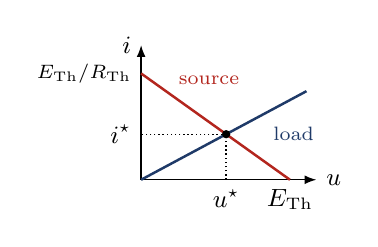
\begin{tikzpicture}[line width=0.5pt, font=\small, x=0.84cm, y=0.9cm]
  \draw[->] (0,0) -- (2.65,0) node[right] {$u$};
  \draw[->] (0,0) -- (0,1.9) node[left] {$i$};
  \draw[trapred, line width=0.9pt] (0,1.5) -- (2.25,0);
  \draw[navy, line width=0.9pt] (0,0) -- (2.5,1.25);
  \fill (1.2857,0.6429) circle (1.5pt);
  \draw[densely dotted] (1.2857,0) -- (1.2857,0.6429) -- (0,0.6429);
  \node[below] at (1.2857,0) {$\ust$};
  \node[left] at (0,0.6429) {$\ist$};
  \node[below] at (2.25,0) {$\ETh$};
  \node[left, font=\scriptsize] at (0,1.5) {$\ETh/\RTh$};
  \node[trapred, font=\scriptsize, anchor=south west] at (0.42,1.2) {source};
  \node[navy, font=\scriptsize, anchor=north west] at (1.85,0.88) {load};
\end{tikzpicture}
\end{minipage}\hfill
\begin{minipage}[c]{0.51\linewidth}
\textcolor{trapred}{\textbf{Source}} (generator convention): $u = \ETh - \RTh\, i$, a
line of slope $-1/\RTh$ in the $(u, i)$ plane.\\[3pt]
\textcolor{navy}{\textbf{Load}} (receiver convention): $u = R_c\, i$, a line through
$O$ of slope $1/R_c$.
\end{minipage}
\par\smallskip
The \textbf{operating point} is the actual state of the circuit: the unique pair
$(\ust, \ist)$ that satisfies \emph{both} characteristics. Graphically, it is their
\textbf{intersection}.
\nxt
\bx{24}{Analytical determination:} $R_c\,\ist = \ETh - \RTh\,\ist$, so
\begin{fml}
  $\ist = \dfrac{\ETh}{\RTh + R_c} \qquad
   \ust = R_c\,\ist = \dfrac{R_c}{\RTh + R_c}\,\ETh$
\end{fml}
So $\ust$ is a voltage divider between $\RTh$ and $R_c$.
\begin{itemize}
  \item $R_c \to 0$ (short circuit): $\ust \to 0$ and $\ist \to \ETh/\RTh$; the point
    reaches the $i$ axis.
  \item $R_c \to \infty$ (open circuit): $\ist \to 0$ and $\ust \to \ETh$; the point
    reaches the $u$ axis.
  \item In both cases $P_c = \ust\ist = 0$, so the load power has a maximum in between.
\end{itemize}
\hd{Power balance:} the load receives exactly what the real source delivers,
$P_c = \ust\ist = (\ETh - \RTh\ist)\,\ist = R_c\,{\ist}^2$, and
\begin{fml}
  $\underbrace{\ETh\,\ist}_{\text{produced by ideal source}}
   = \underbrace{\RTh\,{\ist}^2}_{\text{lost in } \RTh}
   + \underbrace{R_c\,{\ist}^2}_{\text{received by load}}$
\end{fml}
\hd{Efficiency:}
\begin{fml}
  $\eta = \dfrac{P_c}{\ETh\,\ist} = \dfrac{R_c}{\RTh + R_c} = \dfrac{\ust}{\ETh}$
\end{fml}
It increases with $R_c$: $0$ on short circuit, close to 1 for $R_c \gg \RTh$, and
exactly $\tfrac12$ at $R_c = \RTh$.
\end{panel}
\end{column}\hfill
% ================================================================ page 2, right column
\begin{column}
\begin{panelc}
\hd{Maximum power -- matching:}
\begin{fml}
  $P_c = \dfrac{R_c\,\ETh^2}{(\RTh + R_c)^2} \qquad
   \dfrac{\mathrm{d}P_c}{\mathrm{d}R_c} = \ETh^2\,\dfrac{\RTh - R_c}{(\RTh + R_c)^3}$
  \\[3pt]
  $R_c = \RTh \;\Longrightarrow\; P_c^{\max} = \dfrac{\ETh^2}{4\RTh}$, \quad
  $\eta = 50\,\%$
\end{fml}
\begin{center}
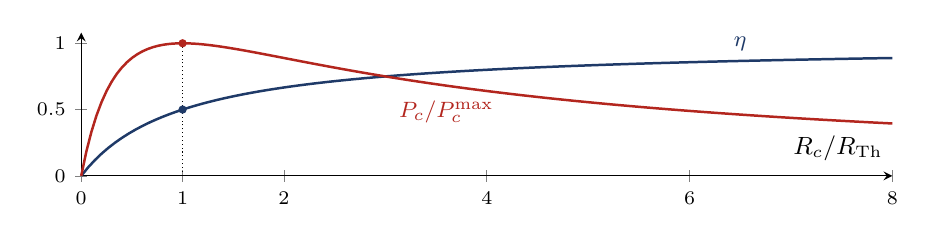
\begin{tikzpicture}
\begin{axis}[width=0.98\linewidth, height=3.4cm, xmin=0, xmax=8, ymin=0, ymax=1.08,
    axis lines=left, xtick={0,1,2,4,6,8}, ytick={0,0.5,1},
    tick label style={font=\scriptsize}, label style={font=\small},
    xlabel={$R_c/\RTh$}, xlabel style={at={(axis description cs:1,0)},
    anchor=south east, yshift=2pt}, clip=false]
  \addplot[navy, line width=0.9pt, domain=0:8, samples=120] {x/(1+x)};
  \addplot[trapred, line width=0.9pt, domain=0:8, samples=160] {4*x/(1+x)^2};
  \draw[densely dotted] (axis cs:1,0) -- (axis cs:1,1);
  \fill[trapred] (axis cs:1,1) circle (1.5pt);
  \fill[navy] (axis cs:1,0.5) circle (1.5pt);
  \node[navy, font=\footnotesize, anchor=south] at (axis cs:6.5,0.87) {$\eta$};
  \node[trapred, font=\footnotesize, anchor=north] at (axis cs:3.6,0.64)
    {$P_c/P_c^{\max}$};
\end{axis}
\end{tikzpicture}
\end{center}
\textbf{Maximum power $\neq$ maximum efficiency}, and no load gives both. Match
($R_c = \RTh$) when the available power is tiny (antenna, sensor, amplifier stage).
Favour efficiency ($R_c \gg \RTh$) when energy is costly and losses cause heating
(power lines, power supplies, a battery driving a motor).
\nxt
\hd{Example:} $\ETh = \qty{10}{V}$, $\RTh = \qty{2.0}{\ohm}$, $R_c = \qty{3.0}{\ohm}$
give $\ist = \qty{2.0}{A}$, $\ust = \qty{6.0}{V}$ and $P_c = \qty{12}{W}$. The ideal
source produces $\qty{20}{W}$ and $\qty{8.0}{W}$ is lost in $\RTh$, so $\eta = 60\,\%$.
With a matched load ($R_c = \qty{2.0}{\ohm}$): $P_c^{\max} = \qty{12.5}{W}$, but
$\eta = 50\,\%$.
\end{panelc}

\begin{panel}{Which tool? \& exam traps}
\begin{itemize}
  \item One unknown potential (a node joined by resistors) $\to$ \textbf{Millman}.
  \item Two resistors in series sharing a voltage $\to$ \textbf{voltage divider}; in
    parallel sharing a current $\to$ \textbf{current divider}.
  \item A load studied while the rest stays fixed $\to$ \textbf{Thévenin} or
    \textbf{Norton}, then the \textbf{operating point}.
  \item Anything else $\to$ \textbf{Kirchhoff}: $N-1$ node laws and $B-N+1$ mesh laws.
\end{itemize}
\begin{trap}
\begin{itemize}
  \item A divider needs the \textbf{same current} in both resistors: with a load,
    combine $R_2 \parallel R_L$ first.
  \item Millman: a branch to ground keeps its $1/R_k$ in the denominator; a reversed
    source counts as $-E_k$.
  \item Sources off: voltage source $\to$ wire, current source $\to$ open. Never remove
    a resistor.
  \item In open circuit, a resistor in series with terminal $A$ carries no current: it
    changes $\RTh$, not $\ETh$.
  \item $u = \ETh - \RTh\, i$ assumes $i$ leaves by $A$ (generator convention). State
    your conventions.
  \item $\eta = P_c/(\ETh\ist)$, not $P_c/P_c^{\max}$.
  \item ``State a law or theorem'': give the words, the diagram or equation, and the
    method for each parameter (that is how the marks are split).
  \item Sanity checks: series $\Req >$ largest $R$; parallel $\Req <$ smallest $R$;
    $V_O$ lies between the $V_k$; $0 \le \eta < 1$.
\end{itemize}
\end{trap}
\hd{Units:} $\unit{\kilo\ohm} \times \unit{mA} = \unit{V}$; \
$\unit{V}/\unit{\kilo\ohm} = \unit{mA}$; \ $\unit{V^2}/\unit{\ohm} = \unit{W}$; \
$\unit{S} = \unit{\ohm^{-1}}$.
\nxt
\hd{Handout notes:} p.~27, eqs.~(15)--(16): the left-hand side is $u_2$ (the voltage
across $R_2$), not $u_1$, and ``$0.9901\,E$'' means $0.9901\,u$. p.~28, eq.~(17): the
denominator is $1/R_1 + 1/R_2 + \dots + 1/R_n$. p.~37, eq.~(24): $P_{\mathrm{Th}}$ there
means $\ETh\ist$ (produced by the ideal source), not the delivered power of eq.~(19).
\end{panel}
\end{column}

\end{document}
